\section{Design Front-end}
In questo capitolo sono illustrati alcuni mockup, relativi alle schermate dell'applicazione web da realizzare. Queste schermate hanno l'obbiettivo di rappresentare come l'applicazione si dovrà presentare nel caso dei seguenti requisiti funzionali:
\begin{itemize}
    \item Fig:\ref{fig:schermata_signup} Registrazione;
    \item Fig:\ref{fig:schermata_login} Login con credenziali e con google;
    \item Fig:\ref{fig:schermata_gioca_single-player} Single-player;
    \item Fig:\ref{fig:schermata_quiz_1} Quiz tipo 1;
    \item Fig:\ref{fig:schermata_quiz_2} Quiz tipo 2;
    \item Fig:\ref{fig:schermata_quiz_3} Quiz tipo 3;
    \item Fig:\ref{fig:schermata_quiz_4} Quiz tipo 4;
    \item Fig:\ref{fig:schermata_gioca_multiplayer} Multiplayer;
    \item Fig:\ref{fig:schermata classifica} Visualizzazione classifica.
\end{itemize}
Pagina principale dell'applicazione:
\begin{figure}[!h]
\centering
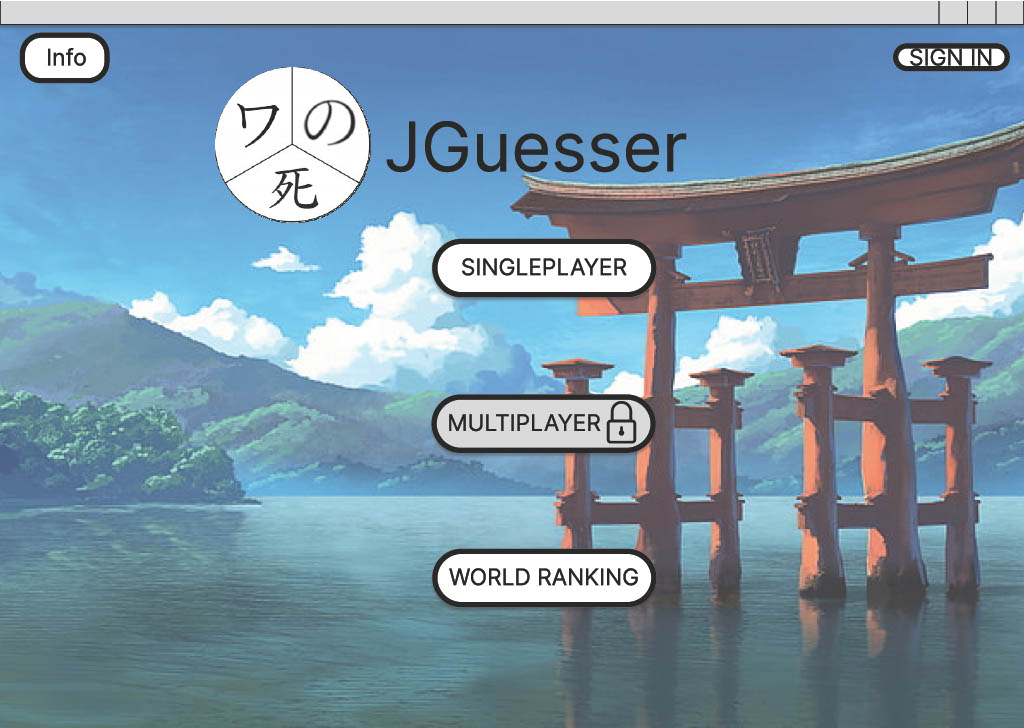
\includegraphics[scale=0.35]{images/home_page.jpg}
\end{figure}

In questa pagina sono visualizzati cinque pulsanti:
\begin{itemize}
    \item info: porta l'utente alla pagina dove potrà visualizzare gli alfabeti Hiragana, Katakana e Kanji e una breve descrizione, con relativa storia. Si fa riferimento al requisito funzionale \ref{req_compendio}.
    \item sign-in: porta l'utente alla pagina per effettuare il login. Vedere Fig:\ref{fig:schermata_login}.
    \item single-player: aprirà un'altra mini finestra, che permetterà all'utente di scegliere se giocare, con uno o più degli alfabeti a sua scelta oppure alla sfida giornaliera. Vedere Fig:\ref{fig:schermata_gioca_single-player}.
    \item multiplayer: aprirà un'altra mini finestra, che permetterà all'utente di scegliere se sfidare un giocatore a sua scelta, tramite username oppure un giocatore casuale. Vedere Fig:\ref{fig:schermata_gioca_multiplayer}.
    \item world ranking: porta l'utente alla pagina dove potrà visualizzare la classifica mondiale. Vedere Fig:\ref{fig:schermata classifica}.
\end{itemize}

\begin{figure}[!h]
\centering
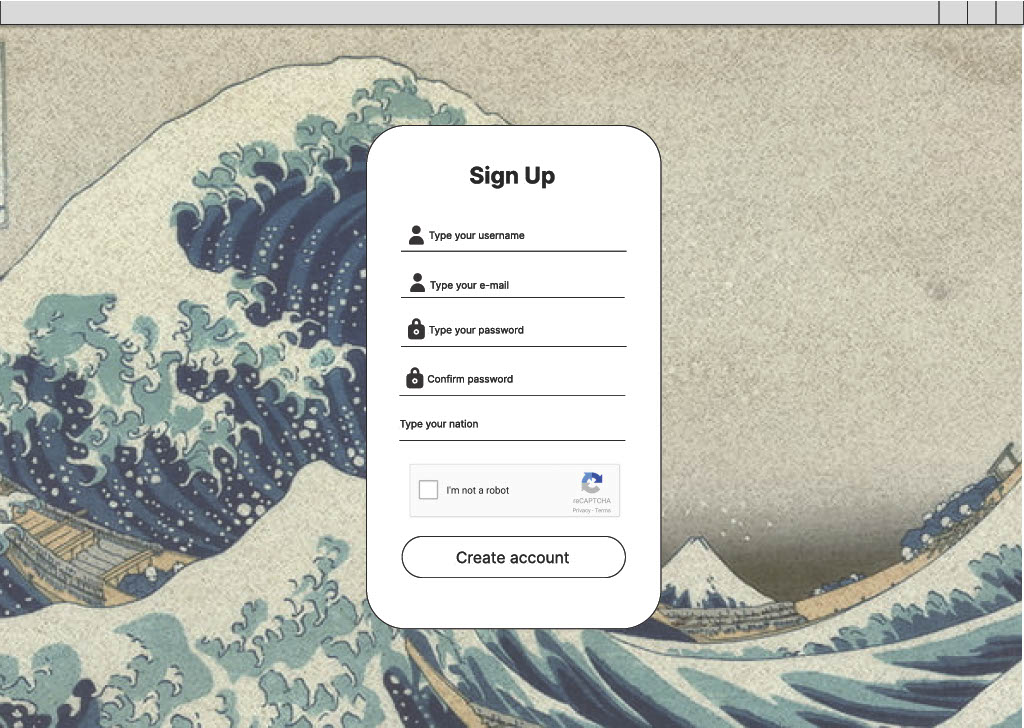
\includegraphics[scale=0.35]{images/signup.jpg}
\caption{Schermata sign-up}
\label{fig:schermata_signup}
\end{figure}
\noindent 
L'utente compila il form richiesto per registrarsi, dove dovrà inserire: e-mail, username, due volte la password e la propria nazione, dopodichè cliccando prima sul reCAPTCHA e poi sul pulsante 'create account' crea il proprio account. Si fa riferimento al requisito funzionale \ref{req_registrazione}. \\
\newpage

\begin{figure}[!h]
\centering
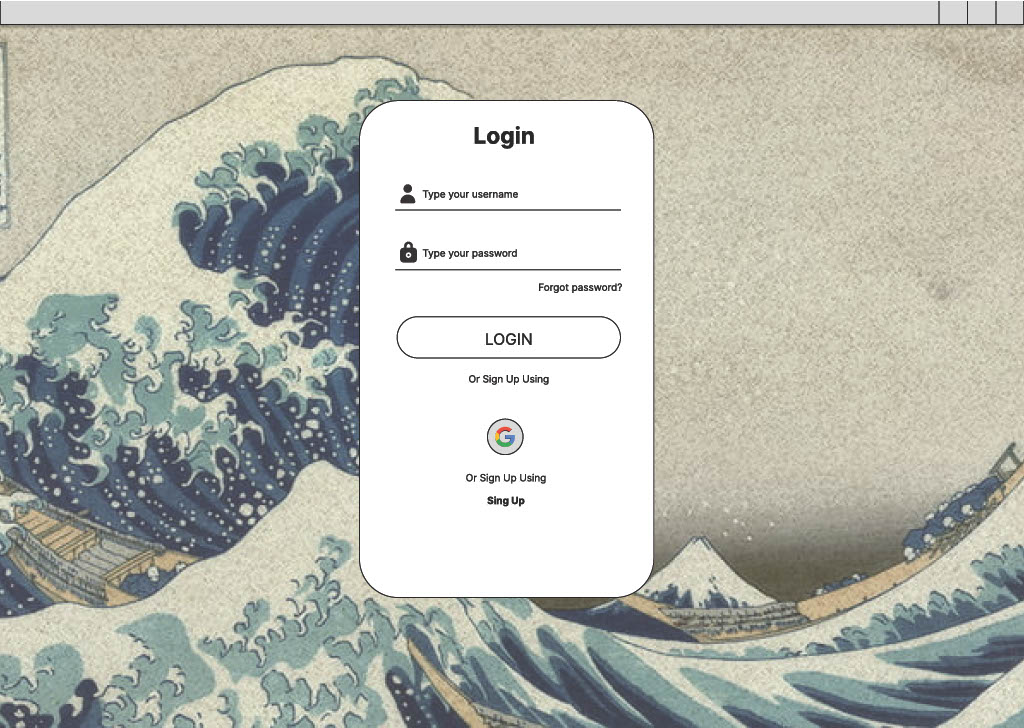
\includegraphics[scale=0.35]{images/login.jpg}
\caption{Schermata login}
\label{fig:schermata_login}
\end{figure}
\noindent 
L'utente potrà compilare il form dove dovrà inserire: username e password per accedere al proprio account, oppure nel caso non ne abbia uno avrà la possibilità di registrarsi attraverso una relativa pagina di sing-up (vedere Fig:\ref{fig:schermata_signup}). La registrazione può avvenire sia tramite l'inserimento di credenziali, ma anche utilizzando un account google. Si fa riferimento ai requisiti funzionali \ref{req_login_con credenziali} e \ref{req_login_con_google}.

\begin{figure}[!h]
\centering
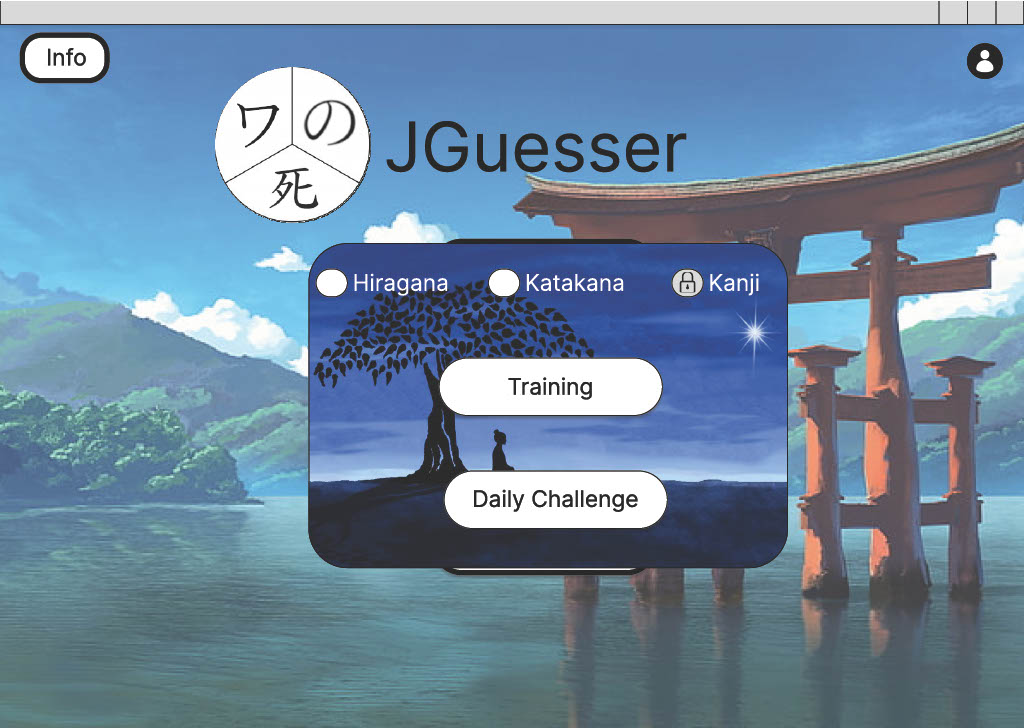
\includegraphics[scale=0.35]{images/single-player.jpg}
\caption{Schermata single-player}
\label{fig:schermata_gioca_single-player}
\end{figure}
\noindent
Questa schermata rappresenta la pagina di single-player. All'utente saranno date due possibilità. Egli potrà scegliere se allenarsi con un insieme di alfabeti a sua scelta, oppure potrà decidere di provare la sfida giornaliera. Si fa riferimento al gruppo di requisiti funzionali \ref{req_scegli_modalità_single_player}.

\begin{figure}[!h]
\centering

\includegraphics[scale=0.35]{images/quiz_1.jpg}
\caption{Schermata quiz tipo 1}
\label{fig:schermata_quiz_1}
\end{figure}
\noindent
Questo è come si dovrebbe presentare il quiz di tipo 1. Cliccando sul pulsante 'home' in alto a sinistra, l'utente potrà terminare la propria sessione di gioco, cliccando invece sul pulsante score l'utente potrà visualizzare una serie di statistiche temporanee. Si fa riferimento ai requisiti funzionali \ref{req_quiz_1}, \ref{req_termina_sessione_di_gioco} e \ref{req_risultato_score}.
\newpage

\begin{figure}[!h]
\centering
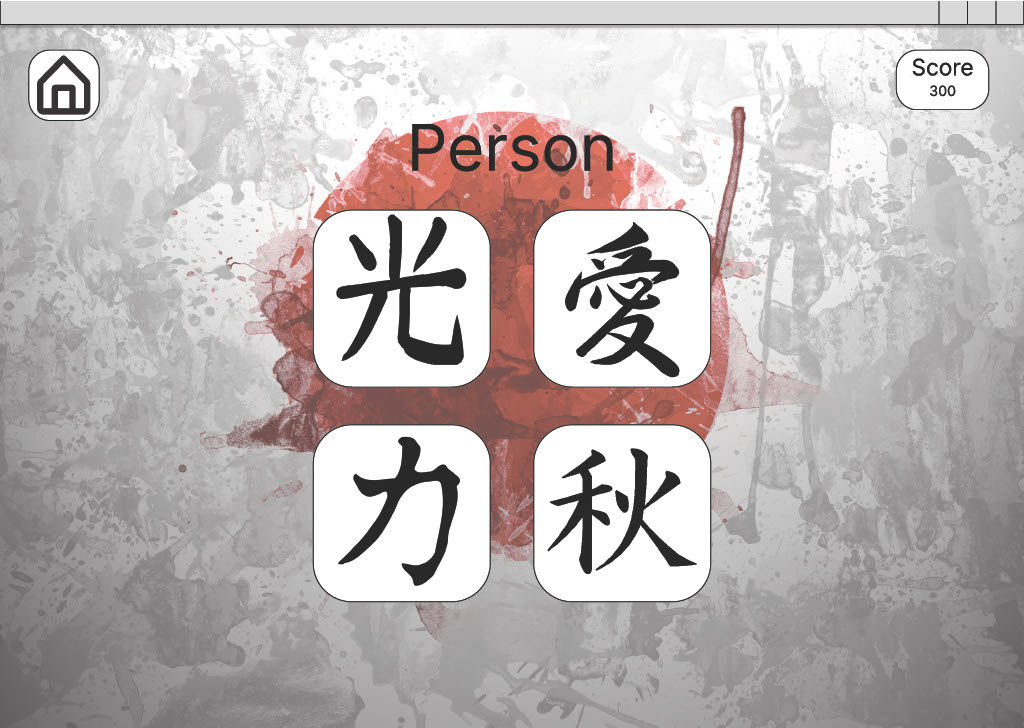
\includegraphics[scale=0.35]{images/quiz_2.jpg}
\caption{Schermata quiz tipo 2}
\label{fig:schermata_quiz_2}
\end{figure}
\noindent
Questo è come si dovrebbe presentare il quiz di tipo 2. Si fa riferimento ai requisiti funzionali \ref{req_quiz_2}, \ref{req_termina_sessione_di_gioco} e \ref{req_risultato_score}.

\begin{figure}[!h]
\centering
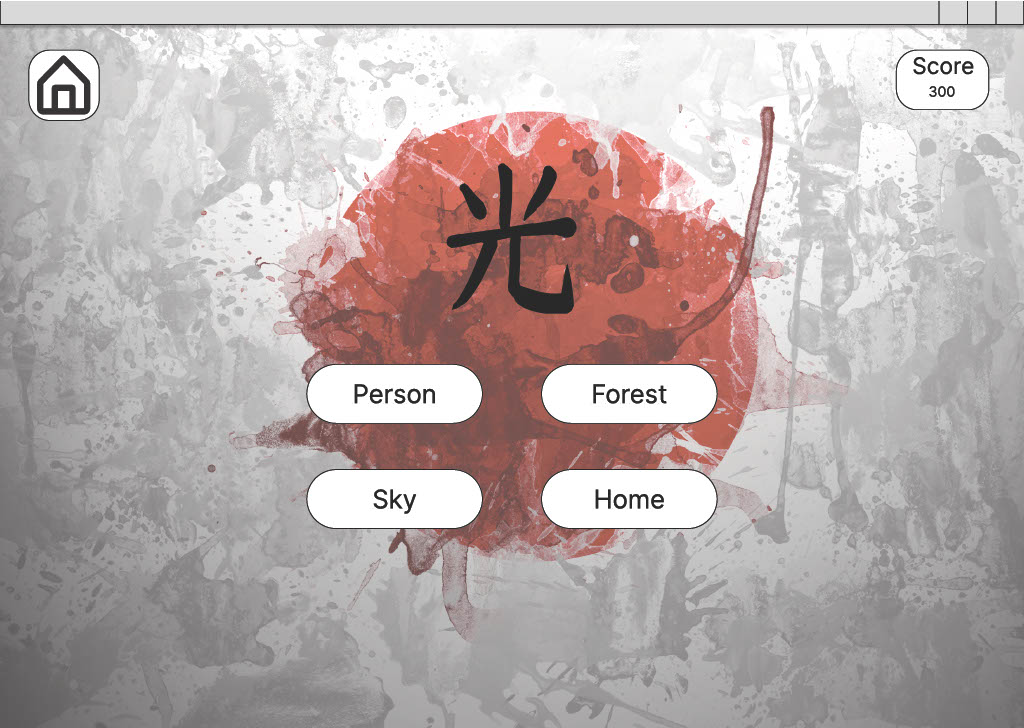
\includegraphics[scale=0.35]{images/quiz_3.jpg}
\caption{Schermata quiz tipo 3}
\label{fig:schermata_quiz_3}
\end{figure}
\noindent
Questo è come si dovrebbe presentare il quiz di tipo 3. Si fa riferimento ai requisiti funzionali \ref{req_quiz_3}, \ref{req_termina_sessione_di_gioco} e \ref{req_risultato_score}.
\newpage

\begin{figure}[!h]
\centering
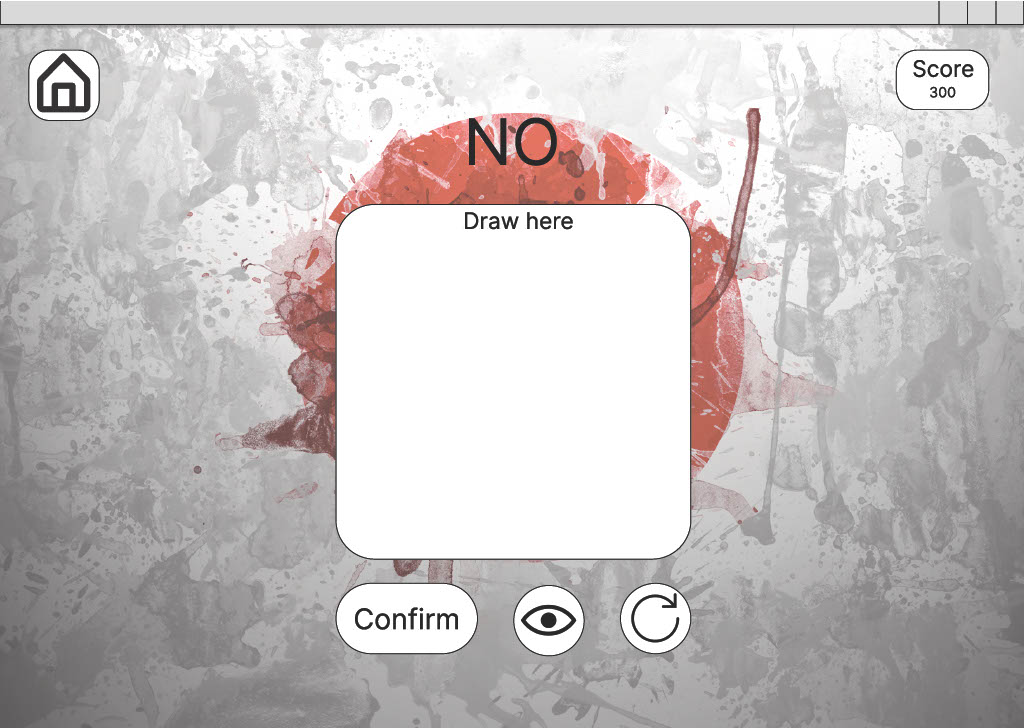
\includegraphics[scale=0.35]{images/quiz_4.jpg}
\caption{Schermata quiz tipo 4}
\label{fig:schermata_quiz_4}
\end{figure}
\noindent
Questo è come si dovrebbe presentare il quiz di tipo 4. Si fa riferimento ai requisiti funzionali \ref{req_quiz_4}, \ref{req_termina_sessione_di_gioco} e \ref{req_risultato_score}.

\begin{figure}[!h]
\centering
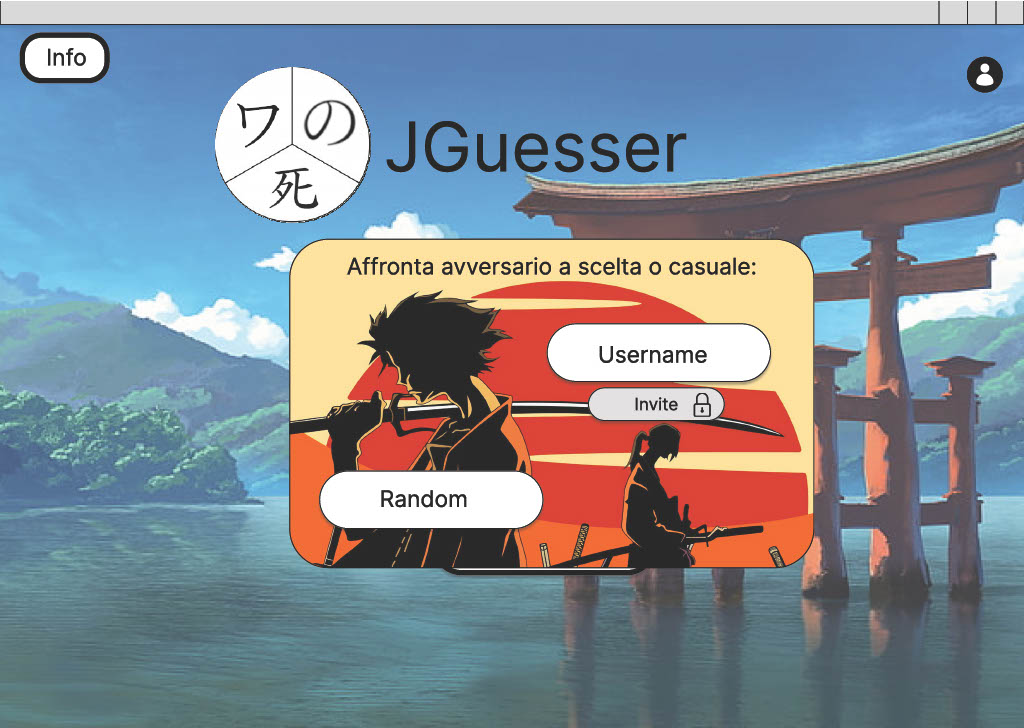
\includegraphics[scale=0.35]{images/multiplayer.jpg}
\caption{Schermata multiplayer}
\label{fig:schermata_gioca_multiplayer}
\end{figure}
\noindent
Questa schermata rappresenta la pagina di multiplayer. L'utente potrà decidere se affrontare uno specifico giocatore, inserendo il proprio username in un form e cliccando sul pulsante 'join', oppure potrà scegliere di sfidare un giocatore casuale cliccando sul pulsante 'random'. Si fa riferimento al gruppo di requsiti funzionali \ref{req_multiplayer}.

\begin{figure}[!h]
\centering
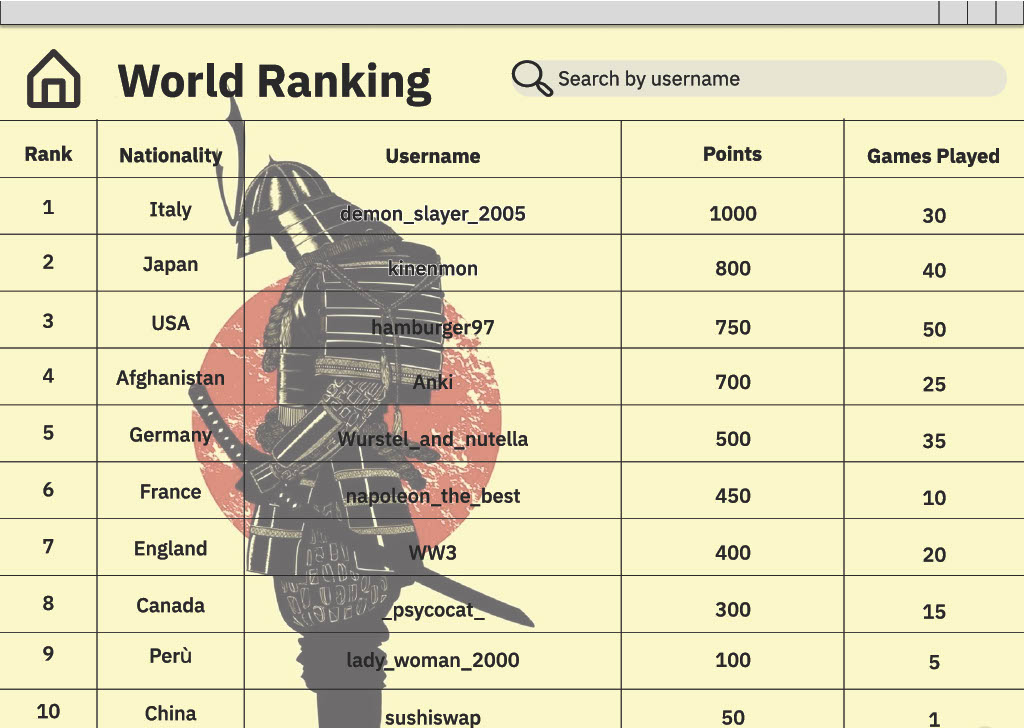
\includegraphics[scale=0.35]{images/world_ranking.jpg}
\caption{Schermata classifica}
\label{fig:schermata classifica}
\end{figure}
\noindent
Questa pagina rappresenta la classifica mondiale, che qualsiasi utente potrà visualizzare. Per ogni utente è visualizzato il proprio rank, nazionalità, username, punti (guadagnati finora) e il numero di partite giocate. L'utente potrà grazie ad una barra di ricerca, filtrare uno fra i tanti giocatori della classifica per username. Si fa riferimento ai requisiti funzionali \ref{req_visualizza_classifica} e \ref{req_ricerca_classifica}. 



